\documentclass[a4paper,13pt]{article}
\usepackage[left=1cm,right=1cm,top=1.5cm,bottom=1.5cm,includeheadfoot]{geometry}
\usepackage[utf8]{inputenc}
\usepackage[table]{xcolor}
\usepackage{pdfpages}
\usepackage[pdfborderstyle={/S/U/W 1},colorlinks=true, linkcolor=blue]{hyperref}
\usepackage{longtable}
\usepackage{luacode}

\xdefinecolor{TableLightGray}{rgb}{0.90,0.90,0.90}


\hypersetup{
 pdftitle={LXI/SCPI Example in lualatex},
 pdfauthor={Roman Pollak},
 pdfsubject={Example}
}


\directlua{package.cpath = "./lxit.so" }
\directlua{drv=require("lxit")}


\begin{document}

\title{\Huge{LXI/SCPI Example in LuaLaTeX}}
\date{\today}
\maketitle


\begin{luacode*}




  function meas(con_ko,con_ps,file,max_v,max_i)
  call_scpi(dev_ps,":OUTPut:STATe CH3, ON")
  for v=.3,max_v,.01 do
  call_scpi(con_ps,string.format(":APPLy CH3,%.2fV, 0.02A",v))
  lxi_msleep(1200)
     volt=tonumber(lxi_scpi(con_ps,":SOUR3:VOLT?"))
     val=tonumber(lxi_scpi(con_ko,":DMM:VALue?"))
     if val > max_i then
     lxi_scpi(con_ps,":OUTPut:STATe CH3, OFF")
     file:flush()
     return
     end
     print(string.format("V %.4f I %f \n",volt,val))
     file:write(string.format("V %.4f I %f \n",volt,val))
     --lxi_sleep(1)
  end
  call_scpi(con_ps,":OUTPut:STATe CH3, OFF")
  call_scpi(con_ps,string.format(":APPLy CH3,0.0V, 0.0A"))
  file:flush()
  end

  

 function conv_m(text)

 text=string.gsub(text,"&#39","\\verb|'|")
 text=string.gsub(text,"&#40","(")
 text=string.gsub(text,"&#41",")")
 text=string.gsub(text,"&","\\verb|&|")
 text=string.gsub(text,"#","\\verb|#|")
 text=string.gsub(text,"_","\\textunderscore{}")
 --text=string.gsub(text,"^","\\verb|^|")
 text=string.gsub(text,"/","/\\allowbreak{}")
 --text=string.gsub(text,"%c","")
 test=string.gsub(text,"\026","")

return text
end


function split_string(inputstr, sep)
    if sep == nil then
        sep = "%s"
    end
    local t = {}
    for part in string.gmatch(inputstr, "([^" .. sep .. "]+)") do
        table.insert(t, part)
    end
    return t
end

function text_prompt(msg)
  io.write(msg)
  io.flush()
  return io.read()
end

function call_scpi(con,msg)
lxi_scpi(con,msg)
err_msg=lxi_scpi(con,"SYSTem:ERRor?")
print(err_msg .. "On ".. msg)
end

--addr=text_prompt("Please give the Name or IP Address of the LXI/SCPI Device? :")


  tex.sprint("\\section{Measurement Equipment}")
  tex.sprint("\\rowcolors{2}{TableLightGray}{white}")
  tex.sprint("\\begin{longtable}{p{5cm}p{7cm}}")
  tex.sprint("\\\\")
  addr="KO"
dev_ko=lxi_connect(addr,nil, nil, 2000, "RAW")
dev_id=lxi_scpi(dev_ko,"*IDN?")
print(dev_id)
result=split_string(dev_id,",")
print(result)
  tex.sprint("Device Manufacturer & " .. conv_m(result[1]) .. "\\\\")
  tex.sprint("Model & " .. conv_m(result[2]) .."\\\\")
  tex.sprint("Serial Nr. & " .. conv_m(result[3]) .. "\\\\")
  tex.sprint("Firmware & " .. conv_m(result[4]) .. "\\\\")
addr="PS"
dev_ps=lxi_connect(addr,nil, nil, 2000, "RAW")
dev_id=lxi_scpi(dev_ps,"*IDN?")
print(dev_id)
result=split_string(dev_id,",")
print(result)
  tex.sprint("Device Manufacturer & " .. conv_m(result[1]) .. "\\\\")
  tex.sprint("Model & " .. conv_m(result[2]) .."\\\\")
  tex.sprint("Serial Nr. & " .. conv_m(result[3]) .. "\\\\")
  tex.sprint("Firmware & " .. conv_m(result[4]) .. "\\\\")
  
  tex.sprint("\\end{longtable}")


  print("Setup Measurement")
 -- call_scpi(dev_ko,":POWERS:OUTP1:VOLT 1")
 -- call_scpi(dev_ko,":POWERS:OUTP1 ON")
  lxi_scpi(dev_ko,":DMM:STATE ON")
  lxi_scpi(dev_ko,":DMM:MODe DCMA")
 
  lxi_sleep(2)


 

     ask= text_prompt("Redo Measurements [Y/N]")
     if ask == "Y" then 
     
     file = io.open ("led_data.dat", "w")
     led={"1N4148","Ir","Red","Yellow","Green","Blue","White","Uv"}
     for a in pairs(led)
     do
     text_prompt("Ready to meassure "..led[a].." Led?")
     file:write(string.format("\"%s LED\"\n",led[a]))
     meas(dev_ko,dev_ps,file,4,.020)
     file:write("\n\n")
     end
     file:close()
     end

     tex.sprint("\\section{Measurements}")
 

     gp_text=[[
         set terminal pdfcairo color size 17cm,10cm
         set colorsequence classic
         set title "LED/Diode Characteristics"
         set grid
         set ylabel "Current (A)"
         set xlabel "Voltage (V)"
         plot for [i=0:*] "led_data.dat" index i using 2:4 smooth bezier w l title columnhead(1)
     ]]

     gp_prg=io.popen ("gnuplot","w")
     gp_prg:write("set output \"./led_data.pdf\"\n")
     gp_prg:write(gp_text)
     gp_prg:flush()
     gp_prg:close()

     file1=io.open("./led_data.pdf","r")
     if file1 ~= nil then
     size=file1:seek("end")
     print(size)
     if size > 0 then
     
     tex.sprint("\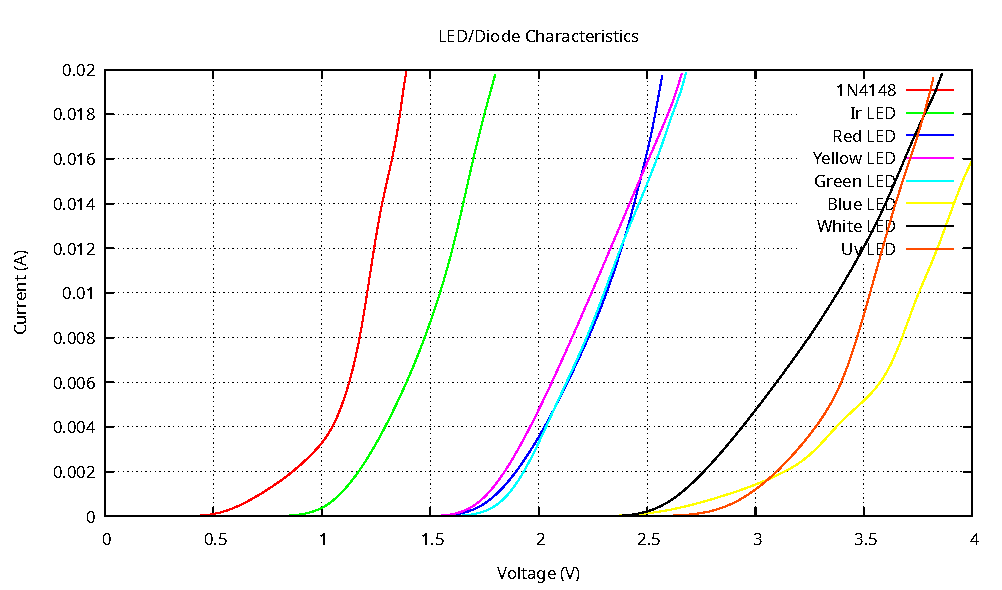
\includegraphics[scale=1]{led_data}")
     file1:close()
     end
     end
tex.sprint("\\\\")
     
\end{luacode*}



\end{document}

